\documentclass[nostrict]{szablonPG}

%-------------------- Dodatkowe pakiety ---------------------
% komendy usepackage
%------------------------------------------------------------

%------------------------------------------------------------
%			      Poczatek pracy dyplomowej  
%------------------------------------------------------------

\begin{document}

%------------------------------------------------------------
%  Dodanie strony tytulowej wygenerowanej z MojaPG oraz 
%  						oswiadczenia

%\includepdf{meta/strona_tytulowa.pdf}
%\includepdf{meta/oswiadczenie.pdf}

%------------------------------------------------------------
%  Dodanie streszczenia i abstract
%  						

\chapter*{Streszczenie}
\indent W poni�szej pracy opisano etapy budowania platformy edukacyjnej wykorzystuj�cej szeroko poj�te mechanizmy grywalizacji, nazywan� zamiennie gamifikacj�. W pierwszym rozdziale om�wiono wst�p i cel pracy. W drugim rozdziale przedstawiono g��wne mechanizmy grywalizacji oraz tematyk� kursu realizowanego w ramach studium przypadku. W trzecim rozdziale dokonano przegl�du istniej�cych rozwi�za� w obszarze zdalnego nauczania i wykorzystywania mechanizm�w gamifikacji. W kolejnym opisano analiz� projektowanego systemu. Zawarto w nim takie elementy jak wizja systemu, diagramy przypadk�w u�ycia i diagram klas. W pi�tym rozdziale opisano projekt systemu, czyli metodyk� pracy, architektur� ca�ego systemu oraz przedstawiono schemat bazy danych. W sz�stym i si�dmym rozdziale opisano szczeg�y implementacji wybranych fragment�w systemu oraz studium przypadku. W ko�cowym rozdziale przedstawiono wnioski i spostrze�enia w postaci podsumowania.\vspace{0.5cm}\newline

\noindent \textbf{S�owa kluczowe:} gamifikacja, nauczanie zdalne, diagramy UML, serwis internetowy\vspace{0.5cm}\newline
\noindent \textbf{Dziedzina nauki i techniki, zgodnie z wymogami OECD:} Informatyka
\chapter*{Abstract}
\indent The following paper describes the stages of building an educational platform that uses the mechanisms of gamification, interchangeably called gamification. The first chapter discusses the introduction and purpose of the paper. The second chapter presents the main mechanisms of gamification and the subject matter of the case study course. The third chapter reviews existing solutions in the area of remote learning and the use of gamification mechanisms. The next one describes the analysis of the designed system. It includes elements such as system vision, use case diagrams and class diagram. The fifth chapter describes the system design, i.e. the working methodology, the architecture of the whole system, and presents the database schema. The sixth and seventh chapters describe implementation details of selected parts of the system and a case study. The final chapter presents conclusions and insights in the form of a summary. \vspace{0.5cm}\newline

\noindent \textbf{Keywords:} gamification, remote learning, UML diagrams, web service\vspace{0.5cm}\newline
\noindent \textbf{Field of science and technology, as required by the OECD: } Computer Science

%------------------------------------------------------------
%	Utworzenie spisu tresci pracy dyplomowej
\tableofcontents

%------------------------------------------------------------
%	Dodanie wykazu wazniejszych skrotow i oznaczen 
\chapter*{Wykaz wa�niejszych oznacze� i skr�t�w}
\addcontentsline{toc}{chapter}{Wykaz wa�niejszych oznacze� i skr�t�w}

 
API -- Application Programming Interface 

ABI -- Application Binary Interface 


%------------------------------------------------------------
%	Dodanie rozdzialoww pracy dyplomowej - glowne cialo dokumentu 

\chapter{Wst�p}

\chapter{Przegl�d podobnych system�w}

\chapter{Wymagania wzgl�dem systemu}
\section{Wizja systemu}

\section{Opis dziedziny problemowej}

\subsection{Poj�cie gamifikacji}

Gamifikacja bywa te� nazywana grywalizacj� i jest ona u�yciem element�w gier i technik projektowania gier w kontek�cie nie zwi�zanymi z grami. Nazwa tego podej�cia pochodzi od tego, �e to przemys� gier by� pionierem w tej dziedzinie, bo gry nie maj� innego celu, ni� zadowolenie osoby w nie graj�cej \cite{deterding}. Wart podkre�lenia jest tutaj fakt, i� gamifikacja w edukacji nie powinna by� rozumiana jako wykorzystanie gier w procesie dydaktycznym. Gamifikacja to raczej metoda, dzi�ki kt�rej zwi�ksza si� zaanga�owanie student�w poprzez obj�cie szerokiego zakresu czynno�ci edukacyjnych, systemem, kt�ry ma motywowa� i jest w du�ej mierze zbli�ony do przebiegu gry. Przyk�adowo podczas prowadzenia gamifikacji na uczelni wy�szej zalecane jest, aby zapewni� studentom \cite{mochocki}

\begin{itemize}
\item kilka �cie�ek do sukcesu (zaliczenia przedmiotu)
\item realn� mo�liwo�� pora�ki (niezaliczenie przedmiotu)
\item stopniowe dawkowanie materia�u w miar� post�p�w
\item istnienie element�w losowych, niespodziewanych
\item przejrzyst� map� kursu, ukazuj�c� powi�zanie zada� z celami kszta�cenia
\item epick� formu�a zada�, role/to�samo�ci i narracj� zbudowan� wok� tematyki zaj�� (studenci jako agenci)
\item informacje zwrotne (przyznawane punkty)
\item listy rankingowe wzmacniaj�ce motywacj�
\end{itemize}

Og�lnie rzecz bior�c gamifikacja jest sposobem projektowania, kt�ry k�adzie du�y nacisk na ludzk� motywacj� w procesie i wykorzystuje wszystkie wci�gaj�ce w rozgrywk� mechanizmy, jakie wyst�puj� w grach \cite{octalysis}. Wi�kszo�� system�w skupia si� na funkcjonalno�ci i przypomina sytuacj�, gdzie pracownicy musz� wykonywa� swoj� prac�, bo s� do niej zobowi�zani. Gamifikacja takiemu podej�ciu przeczy i skupia si� w g��wnej mierze na uczuciach i motywacji korzystaj�cych z systemu os�b. 

Wed�ug bada� przeprowadzonych w�r�d student�w Akademii Marynarki Wojennej, kt�rzy korzystali z platformy zbudowanej specjalnie na potrzeby systemu grywalizacji \cite{rodwald}:
\begin{itemize}
\item �rednia liczba student�w uczestnicz�cych w wyk�adach wynosi�a 82\%, co oznacza wzrost 34\% w stosunku do grupy, dla kt�rej przedmiot odbywa� si� bez wykorzystania gamifikacji
\item �rednia liczba student�w oddaj�ce sprawozdania laboratoryjne w dniu zaj�� wynosi 90\%, co stanowi wzrost o 81\% w stosunku do grupy bazowej
\item �rednia liczba student�w bior�cych udzia� w nieobowi�zkowych zadaniach wynosi 82\%, czyli praktycznie wszyscy, kt�rzy uczestnicz� w wyk�adach
\end{itemize}

\subsection{Mechanizmy gamifikacji}

Jeden z pionier�w gamifikacji, Yu-kai Chou opracowa� framework, kt�ry ma pom�c w budowaniu system�w korzystaj�cych z jej mechanizm�w. Wyr�ni� on w nim 8 podstawowych filar�w takiego systemu \cite{octalysis}.

\begin{enumerate}
\begin{figure}[ht]
\centering
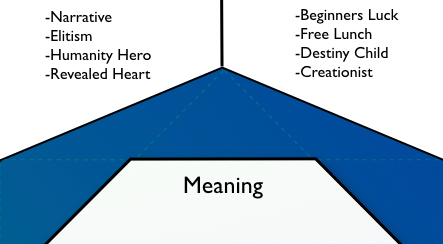
\includegraphics[scale=0.5]{img/chapter2/octalyst1.png}
\caption{Octalyst - epickie znaczenie}
\label{chapter2_octalyst1}
\end{figure}

\item Epickie znaczenie to zasada wedle kt�rej gracz (czy te� ucze�) wierzy �e robi co� wi�cej ni� zwyk�e zadanie zlecone przez nauczyciela. Osoby, kt�re s� cz�onkami  systemu, kt�ry korzysta z tego mechanizmu robi� to nie dlatego, �e praca w nim przynosi im bezpo�rednie korzy�ci, ale dlatego, �e dzi�ki nim staj� si� bohaterami historii wykreowanej po cz�ci przez system i po cz�ci przez nich samych. Przyk�adowe techniki, kt�re wdra�aj� t� zasad� w �ycie:

\begin{itemize}
\item Narracja - wi�kszo�� gier rozpoczyna rozgrywk� od wprowadzenia dlaczego u�ytkownik powinien gra� w t� gr�. Pozwala to wprowadzi� histori�, kt�ra pozwala ludziom zdoby� kontekst, dzi�ki kt�remu s� w stanie nawi�za� lepsz� interakcje z systemem.  
\item Bohater ludzko�ci - technika, kt�ra ma powi�za� dzia�ania podj�te przez u�ytkownik�w z faktem, �e maj� one du�y wk�ad w sprawienie, �e �wiat stanie si� lepszym miejscem. Przyk�adowo firma TOM�s Shoes za wykonane u nich zakupy wysy�a jedn� par� but�w dla dzieci z kraj�w trzeciego �wiata, co sprawia �e robi�c zakupy mamy wra�enie, �e pomagamy ludzko�ci.   
\item Elitaryzm - jest to technika, w kt�rej pozwala si� u�ytkownikom na tworzenie dumnych grup opartych na pochodzeniu etnicznym, przekonaniach, czy zainteresowaniach. Daje im to wra�enie, �e s� cz�ci� wi�kszej sprawy. Przyk�adem mo�e by� rywalizacja pomi�dzy uniwersytetami.
\end{itemize}

\begin{figure}[ht]
\centering
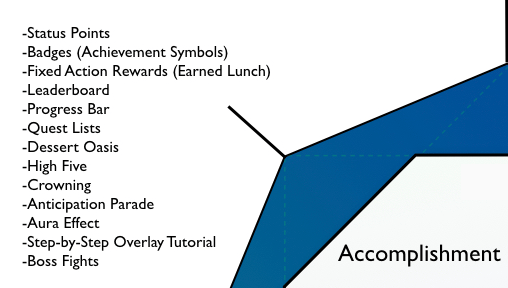
\includegraphics[scale=0.5]{img/chapter2/octalyst2.png}
\caption{Octalyst - rozw�j i osi�gni�cia}
\label{chapter2_octalyst2}
\end{figure}

\item  Rozw�j i osi�gni�cia to zasada, kt�ra prawi o tym, �e rozw�j i osi�gni�cia to wewn�trzny nap�d do robienia post�p�w, rozwijania umiej�tno�ci i ostatecznie pokonywania wyzwa�. Kluczowym sformu�owaniem jest tutaj wyzwanie, gdy� s�owo jest bardzo motywuj�ce przy realizacji zada�. W my�l tej zasady powsta�o wiele prostych w realizacji, ale daj�cych ogromne efekty technik, do kt�rych nale�� mi�dzy innymi:

\begin{itemize}
\item zdobywanie punkt�w
\item ranking lider�w
\item pasek post�pu
\item nagrody (przedmioty, tytu�y)
\end{itemize}

\begin{figure}[ht]
\centering
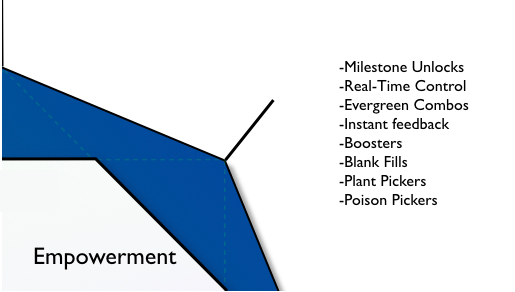
\includegraphics[scale=0.5]{img/chapter2/octalyst3.png}
\caption{Octalyst - wzmocnienie kreatywno�ci}
\label{chapter2_octalyst3}
\end{figure}

\item Wzmocnienie kreatywno�ci to zasada, kt�rej celem jest zbudowanie sytuacji, w kt�rej u�ytkownicy s� zaanga�owani w proces tw�rczy. Przez to s� zobowi�zani do ci�g�ej pracy, w kt�rej musz� my�le� i tworzy� nowe kombinacje. Nale�y r�wnie� pami�ta�, o tym, �e tak samo jak ludzie maj� potrzeb� wyra�ania swojej kreatywno�ci, tak samo maj� potrzeb� by zobaczy� jej efekty.

\begin{itemize}
\item Boosters - technika ta polega na mo�liwo�ci zdobycia przez gracza jakiego� przedmiotu lub zdolno�ci, kt�ra na chwil� drastycznie zwi�ksza jego umiej�tno�ci. Przyk�adowo mo�e to by� mikstura odporno�ci, kt�ra zapewni odporno�� na wszelkie obra�enia a ci�gu minuty od jej wypicia.  
\item Odblokowanie kamienia milowego - technika ta wykorzystuje mechanizm stosowany w grach RPG polegaj�cy na odblokowywaniu nowych umiej�tno�ci wraz ze zdobyciem nowego poziomu. Przyk�adowo przeciwnicy, kt�rzy do tej pory sprawiali nam trudno��, dzi�ki nowo zdobytej umiej�tno�ci s� �atwi do pokonania
\item Plant Picker - jest to technika, kt�re swoje korzenie ma w grze Plants vs Zombies. W gruncie rzeczy chodzi o to, �e u�ytkownik po odblokowaniu kamieni milowych musi wybra� kilka z nich w nadchodz�cej rozgrywce. W pierwowzorze polega�o to na wybraniu kilku odpowiednich ro�lin, kt�re gracz b�dzie m�g� wykorzysta� w rozgrywce. 
\end{itemize}

\begin{figure}[ht]
\centering
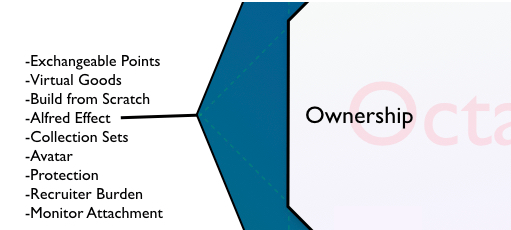
\includegraphics[scale=0.5]{img/chapter2/octalyst4.png}
\caption{Octalyst - w�asno�� i posiadanie}
\label{chapter2_octalys4}
\end{figure}

\item W�asno�� i posiadanie to idea, wed�ug kt�rej u�ytkownicy, kt�rzy s� w�a�cicielami jakich� d�br czuj� si� dobrze w�a�nie dzi�ki temu.  Kiedy gracz jest w�a�cicielem odczuwa pod�wiadomie ch�� sprawienia, by to co posiada sta�o si� lepsze i posiada� co raz wi�cej d�br. Przyk�adowe techniki dzia�aj�ce w ramach tej zasady to:

\begin{itemize}
\item Budowanie od podstaw - w technice tej wykorzystuje si� zjawisko zwi�kszenia zaanga�owania poprzez mo�liwo�� udzia�u w procesie ju� na wczesnym etapie. Przyk�adem tutaj mog� by� meble firmy IKEA, do kt�rych ludzie wydaj� si� by� bardziej przywi�zani ni� do takich, kt�re s� drogie i robione na zam�wienie. Powodem nie musi by� tutaj ich cena, ale fakt, �e u�ytkownik sk�ada� je samodzielnie. 
\item Zestawy kolekcjonerskie - jest to jedna na najsilniejszych technik gamifikacyjnych i polega na mobilizowaniu gracza do skompletowania pewnego zestawu przedmiot�w, kt�ry zebrany w ca�o�ci daje du�e poczucie warto�ci. Niejednokrotnie s�yszano o sytuacjach, gdzie karty kolekcjonerskie by�y sprzedawane za setki tysi�cy dolar�w
\end{itemize}

\begin{figure}[ht]
\centering
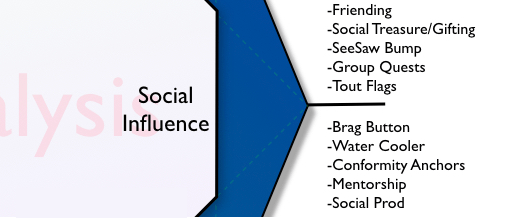
\includegraphics[scale=0.5]{img/chapter2/octalyst5.png}
\caption{Octalyst - relacje spo�eczne}
\label{chapter2_octalyst5}
\end{figure}

\item Relacje i wp�yw spo�eczny w gamifikacji to mechanizm, kt�ry obejmuje wszystkie elementy spo�eczne, kt�re nap�dzaj� ludzi.  Dotyczy to mi�dzy innymi mentoringu, akceptacji, reakcji spo�ecznych oraz konkurencj� i zazdro��. W�r�d wielu technik, kt�re s� w tym obr�bie wykorzystywane na uwag� zas�uguj� mi�dzy innymi:

\begin{itemize}
\item Mentoring - technika ta polega na po��czeniu ze sob� osoby do�wiadczonej i nowicjusza. Obie strony czerpi� w�wczas z tej relacji korzy�ci - nowicjusz zyskuje wiedz� i do�wiadczenie oraz �atwiej mu si� odnale�� w nowym �rodowisku. Weteran z kolei zyskuje pomoc w utrzymaniu zaanga�owania w rozgrywce. 
\item Grupowe zadania - technika ta jest bardzo skuteczna w grze zespo�owej, poniewa� wymaga udzia�u grupy, zanim pojedyncza osoba osi�gnie zwyci�stwo. �wietnym przyk�adem jest tutaj gra World of Warcraft, gdzie mamy dost�p do zada�, kt�re wymagaj� udzia�u zespo�u. Zadania te zmobilizowa�y graczy do tworzenia klan�w, w kt�rych regularnie je wykonuj�. 
\end{itemize}
 
\begin{figure}[ht]
\centering
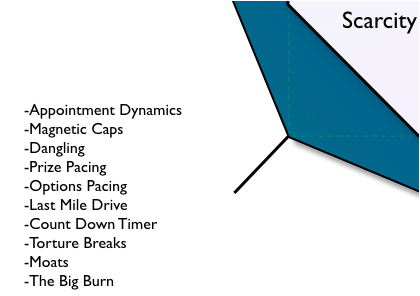
\includegraphics[scale=0.5]{img/chapter2/octalyst6.png}
\caption{Octalyst - niecierpliwo��}
\label{chapter2_octalyst6}
\end{figure} 
 
\item Zasada niedostatku i niecierpliwo�ci wykorzystuje naturalny ludzki nap�d do posiadania czego�, tylko dlatego, ze nie mo�esz tego mie�. Wiele gier wykorzystuje ten mechanizm poprzez odblokowywania nagr�d dopiero po pewnym czasie. Fakt tego, �e nagrod� otrzymamy, ale nie w tym momencie silnie motywuje ludzi i sprawia, �e s� w stanie my�le� o niej przez ca�y dzie�. Przyk�adowe techniki to:

\begin{itemize}
\item Dynamika spotka� to technika, kt�ra wykorzystuje wcze�niej zadeklarowany lub powtarzalny czas, w kt�rym u�ytkownicy musz� podj�� po��dane dzia�ania. Tworzy ona wyzwalacz w oparciu o czas. Przyk�adem z �ycia codziennego jest fakt, �e skoro �mieciarka przyje�d�a po �mieci we wtorek rano, motywuje to ludzi do wyniesienia �mieci w�a�nie przed jej przyjazdem.
\item Tortury przerwy - jest to technika, kt�re powstrzymuje u�ytkownika przez zako�czeniem gry i ka�e mu zrobi� przerw� po to by plony mog�y urosn��, czy energia si� odnowi�a.  Zazwyczaj jest ona nag�a zmiana, kt�ra ma sprawi�, �e gracze zaczn� si� niecierpliwi�. 
\end{itemize}

\begin{figure}[ht]
\centering
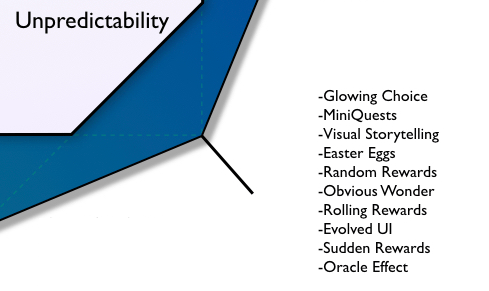
\includegraphics[scale=0.5]{img/chapter2/octalyst7.png}
\caption{Octalyst - nieprzewidywalno��}
\label{chapter2_octalyst7}
\end{figure} 

\item Nieprzewidywalno�� i ciekawo�� wykorzystuje nieszkodliwe d��enie do tego, by dowiedzie� si�, co b�dzie dalej. Dla ludzkiego umys�u naturalnym stanem rzeczy jest my�lenie na temat, tego czego nie wiemy, a wiedzie� chcemy. Niestety nap�d ten jest te� g��wnym czynnikiem uzale�nienia od hazardu, gdy� jest podstaw� organizowania r�nych loterii. Przyk�adowe techniki wykorzystywane w tym obszarze to:

\begin{itemize}
\item Loteria - kluczowym za�o�eniem tej techniki jest zasada i� jak d�ugo pozostaniesz w grze, szanse na wygran� rosn�. Zazwyczaj mamy tutaj niski pr�g wej�cia oraz bardzo du�e nagrody, kt�rych szansa na wygran� jest bardzo niewielka i w du�ej mierze zale�y od szcz�cia. 
\item Easter Eggs - s� to niespodzianki przyznawane bez potwierdzenia przez u�ytkownika. Nagrody s� bardzo niskiej warto�ci, ale sam fakt powodzenia sprawia �e jest przyjemne do�wiadczenie. Dobrym przyk�adem tej techniki mog� by� ukryte wiadomo�ci od os�b tworz�cych dany system.
\item Mistyczne Skrzynki -  technika ta polega na organizowaniu w trakcie rozgrywki losowych nagr�d, kt�re s� wr�czane graczom po uzyskaniu zwyci�stwa. Uczucie jakie towarzyszy u�ytkownikowi podczas otwierania tytu�owej skrzynki jest bardzo zbli�one do tego, co czuj� dzieci podczas rozpakowywania prezent�w wigilijnych. 
\end{itemize}

\begin{figure}[ht]
\centering
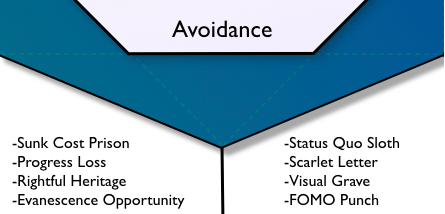
\includegraphics[scale=0.5]{img/chapter2/octalyst8.png}
\caption{Octalyst - unikanie strat}
\label{chapter2_octalyst8}
\end{figure} 

\item unikanie strat - dotyczy unikania negatywnych zjawisk. Mo�e to by� zar�wno strata wykonanej pracy, jak i niemo�no�� wykonania dodatkowych zada�, kt�re mog� wymaga� wi�kszych nak�ad�w pracy.  Przyk�adowe techniki wykorzystuj�ce zasad� unikania strat:

\begin{itemize}
\item Pe�noprawne dziedzictwo - technika ta polega na przekonaniu u�ytkownika, �e co� s�usznie nale�y do niego, a nast�pnie utwierdzeniu go w przekonaniu, �e je�li podejmie niepo��dane dzia�ania, to mo�e to straci�. 
\item Ulotna szansa - to technika polegaj�ce na motywowaniu u�ytkownika do szybkiego dzia�ania w obawie przez utrat� �wietnej oferty. �wietnie sprawdza si� tutaj wykorzystanie licznika czasu, kt�ry jeszcze bardziej zwi�ksza motywacj� u�ytkownika do skorzystania z oferty.
\item Sunk Cost Prison - nazwa tej techniki w j�zyku polskim nazywana jest wi�zieniem utopionych koszt�w. Jest on najbardziej wp�ywow� technik� zasady unikania strat. Wyst�puje w�wczas, gdy u�ytkownik mimo niech�ci, czy braku przyjemno�ci do wykonywania zada� dalej je realizuje, bo nie chce poczu� straty zwi�zanej z porzuceniem wszystkiego. Przyk�adem mo�e by� gra, kt�ra po wielu godzinach nam si� ju� znudzi�a, ale gramy w ni� dalej, bo nie chcemy porzuci� zdobytych w grze d�br. 
\end{itemize}














\end{enumerate}













\section{Wymagania og�lne}
\section{Wymagania dotycz�ce systemu}
\section{Wymagania projektowo wdro�eniowe}
\chapter{Analiza systemu (Marek Grudkowski)}

\section{Model przypadk�w u�ycia}
\section{Model statyczny systemu}
\section{Model dynamiczny systemu}
\chapter{Zagadnienia projektowo-implementacyjne}

Po analizie projektowanego systemu wybrano technologie i rozwi�zania, z kt�rych zesp� b�dzie korzysta� podczas jego implementacji. W przypadku stosowanych rozwi�za� postanowiono w g��wnej mierze opiera� si� na kulturze DevOps i jej rozbudowanych ideach. Je�li chodzi o wykorzystane technologi� system mia� by� zbudowany w oparciu o dwie technologie. Frontend mia� zosta� zbudowany w oparciu o framework React napisany w j�zyku Javascript. Z kolei do backendu mia� zosta� wykorzystany Django - framework napisany w j�zyku skryptowym Python. Aktualnie s� to technologie wysoce popularne na rynku i oferuj�ce wiele rozbudowanych mo�liwo�ci w tworzeniu serwis�w internetowych. 
\section{Architektura systemu}
\section{Projekt bazy danych}
\section{Interfejs u�ytkownika}
\section{Logika biznesowa}
\chapter{Zagadnienia implementacyjne}

\section{Wybrane rozwi�zania}
\section{Instalacja systemu}
\chapter{Studium przypadku}

\chapter{Podsumowanie}



% ---------------------- Bibliografia -----------------------
\bibliographystyle{plain}                       % styl bibliografii
\begin{thebibliography}{3}                      % pocz�tek �rodowiska
\addcontentsline{toc}{chapter}{Wykaz literatury}    % dodaje bibliografi� do spisu tre�ci
\small              % spisy i bibliografie sk�adamy mniejszym stopniem pisma


% rodwald gamifikacja
\bibitem{rodwald}
Rodwald P.: \emph{Gamifikacja � czy to dzia�a?}, EduAkcja. Magazyn edukacji
elektronicznej nr 1 (11)/2016, str. 43�50 

% deterging gamifikacja
\bibitem{deterding}
Deterding S., Dixon D., Khaled R., Nacke L: \emph{From game design elements to
gamefulness: defining gamification}, Proceedings of the 15th International Academic
MindTrek Conference: Envisioning Future Media Environments, Tampere, Finland,
ACM, September 28-30, 2011, 9�15

% mochocki gamifikacja
\bibitem{mochocki}
Mochocki M.: \emph{Gamifikacja szkolnictwa wy�szego - obce wzorce, polskie perspektywy}, Game Industry Trends, Warszawa 2012

% link gamifikacja
\bibitem{octalysis}
Octalysis Complete Gamification Framework, https://yukaichou.com/gamification-examples/octalysis-complete-gamification-framework/ (data dost�pu 20.05.2021 r.).
  
% podrecznik biologia
\bibitem{biologia}
Bonar E., Krzeszowiec-Jele� W., Czachorowski S.: \emph{Biologia na czasie. Podr�cznik dla szk� ponadgimnazjalnych. Zakres Podstawowy.}, Nowa Era, Warszawa 2012

% platforma edukacyjne men
\bibitem{energia} Platforma edukacyjna MEiN, https://zpe.gov.pl/a/zrodla-energii-w-polsce/DZ9m3Dvd0/ (data dost�pu 12.06.2021 r.).

% wolski wymagania jakosciowe
\bibitem{wolskipro}
Blog dotyczacy modelowania UML, M. Wolski, https://wolski.pro/ (data dost�pu 12.09.2021 r.).

% bobkowska wyk�ady
\bibitem{usecase}
Model przypadk�w u�ycia, materia�y wyk�adowe z przedmiotu In�ynieria Oprogramowania, A. Bobkowska, Katedra In�ynierii Oprogramowania, Politechnika Gda�ska, 2020 r. 

% rup package use case
\bibitem{caseuse}
Rational Unified Process. Artifacts, https://sceweb.uhcl.edu/helm/RationalUnifiedProcess/, (data dost�pu 03.10.2021 r.)

% diagram klas 
\bibitem{klasyuml}
Diagramy klas UML, K. Tybulec, https://www.p-programowanie.pl/uml/diagramy-klas-uml (data dost�pu 18.10.2021 r.).

\end{thebibliography}                           % koniec �rodowiska % dodanie pliku bibliografii
% -----------------------------------------------------------

%------------------------------------------------------------
%	Dodanie wykazu rysunkow oraz tabeli

\renewcommand{\baselinestretch}{1.0}\normalsize	% interlinia w sekcji wykazow
\addcontentsline{toc}{chapter}{\listfigurename}	% dodanie wykazu rysunkow do spisu tresci
\listoffigures									% generacja wykazu rysunkow

\addcontentsline{toc}{chapter}{\listtablename}	% dodanie wykazu tabel do spisu tresci
\listoftables									% generacja wykazu tabel
\renewcommand{\baselinestretch}{1.3}\normalsize	% powrot do interlinii 1.5


% ---------------------- DODATKI -----------------------
% \chapter*{Dodatek A}
% \addcontentsline{toc}{chapter}{Dodatek A}
% \includepdf{dodatki/dodatek1.pdf}

% -----------------------------------------------------------
\end{document}
%------------------------------------------------------------
			 	%	Koniec pracy dyplomowej  %
%------------------------------------------------------------
